% DOCUMENT CLASS
\documentclass[11pt]{article}
%PACKAGES
\usepackage[utf8]{inputenc}
\usepackage[ngerman]{babel}
\usepackage[reqno,fleqn]{amsmath}
\setlength\mathindent{10mm}
\usepackage{amstext}
\usepackage{amssymb}
\usepackage{fancyhdr}
\usepackage{units}
\usepackage{comment}  % mehrzeilige Kommentare
\usepackage{cancel} %Brueche kuerzen
\usepackage[table]{xcolor}
\usepackage{tabularx}
\newcolumntype{L}[1]{>{\raggedright\arraybackslash}p{#1}} % linksbündig mit Breitenangabe
\newcolumntype{C}[1]{>{\centering\arraybackslash}p{#1}} % zentriert mit Breiten
% Grafik
\usepackage{graphicx}
\usepackage{subfigure}
\usepackage{wrapfig}
% Zahlenwerte mit Einheiten mittels \unit{Zahlenwert}{Einheit}
\usepackage[thinspace,thinqspace,squaren,textstyle]{SIunits}
% FORMATIERUNG
\usepackage[paper=a4paper,left=25mm,right=25mm,top=25mm,bottom=25mm]{geometry}
\setlength{\parindent}{0cm}
\setlength{\parskip}{1.5mm plus1mm minus1.5mm}
% PAGESTYLE
\pagestyle{fancy}
\setlength\headheight{30pt}
\lhead{Michael Hufschmidt, Mat. Nr. 6436122\\Florian Jochheim, Mat. Nr. 6508131}
\rhead{Übungen zur Physik IV, SoSe 2015\\Blatt 11 zum 06.07.2015}
%MATH SHORTCUTS
\newcommand*{\NN}{\mathbb N}
\newcommand*{\ZZ}{\mathbb Z}
\begin{document}
\begin{comment}
\begin{center}
\begin{tabular}{|L{3cm}|C{1cm}|C{1cm}|C{1cm}|}
\hline
Aufgabe:&\cellcolor{blue!25}24 &\cellcolor{blue!25} 25 &\cellcolor{blue!26} $\sum$\\
\hline
mögliche Punkte: & 5 & 5 & 10 \\
\hline
erreichte Punkte: &  &  & \\
\hline
\end{tabular}
\end{center}
\end{comment}

\subsection*{Aufgabe 24}

\subsubsection*{a)}
Hier auch gleich unsere Formelsammlung für den Spickzettel.
Magnetisierung $\vec M(\vec r, t)$, Magnetfeld $\vec H(\vec r, t)$, und Flußdichte
$\vec B(\vec r, t)$ hängen mit der magnetischen Feldkonstante $\mu_0$ wie folgt zusammen
($V$ = Volumen, $F$ = freie Energie):
\begin{align*}
  [\vec m] = [\vec \mu] &= \frac{\text{J}}{\text{T}} = \text{A m}^2 \qquad \text{magnetisches Moment}\\
  \vec M & = \frac{\vec m}{V} = - n \cdot \left(\frac{\partial F}{\partial B} \right)
  \qquad \text{Magnetisierung = magn. Moment pro Volumen}\\
  [M] = [H] &= \frac{\text{A}}{\text{m}} \\
  \vec M &= \chi \cdot \vec H =  (\mu_r - 1) \vec H
    \;;\quad \vec B = \mu_r \mu_0 \vec H = \mu_0 (\vec H + \vec M) = \mu_0 (1 + \chi)\vec H\\
  \chi & = \mu_r - 1 = \mu_0 \left(\frac{\partial M}{\partial B_{ext}} \right)
  = - \frac{\mu_0}{V}  \left(\frac{\partial^2 F}{\partial B_{ext}^2} \right)_{T, V}
  \qquad \text{magnetische Suszeptibilität}\\
  [B] &= \text{T} = \frac{\text{V s}}{\text{m}^2} \\
  [\mu_0] &= \frac{\text{V s}}{\text{A m}} \\
  [\epsilon_0] &= \frac{\text{A s}}{\text{V m}} \\
  \mu_B &=  \frac{e \hbar}{2 m_e} = 9{,}274 \cdot 10^{-24}\frac{\text{J}}{\text{T}}
    = 9{,}274 \cdot 10^{-24}\text{A m}^2  \qquad \text{Bohrsches Magneton}\\
  k_B &= 1{,}380 \cdot 10^{-23}\frac{\text{J}}{\text{K}}
\end{align*}
Fehler im Skript bei der Formel für $\chi$.

\subsubsection*{b)}
Fehler im Aufgabenzettel bei der Formel für $<\mu>$.
\begin{align}
\nonumber
<\mu> &= \mu_B \cdot \frac{\exp\left(+\frac{\mu_B B}{k_B T}\right) -
 \exp\left(-\frac{\mu_B B}{k_B T}\right)}
  {\exp\left(+\frac{\mu_B B}{k_B T}\right) + \exp\left(-\frac{\mu_B B}{k_B T}\right) } =
  \mu_B \cdot \frac{\sinh\left(\frac{\mu_B B}{k_B T}\right)}{\cosh\left(\frac{\mu_B B}{k_B T}\right)}\\
\intertext{Ein fcc-Gitter enthält  4 Atome pro Elementarzelle (Volumen $= a^3$), also:}
\label{eq-M}
M &= \frac{4 \mu_B}{a^3}\cdot \tanh \left(\frac{\mu_B B}{k_B T}\right)
\intertext{Im Grenzfall $T \rightarrow 0$ ergibt das}
\label{eq-MS}
M_S &= \frac{4 \mu_B}{a^3} = \frac{4 \cdot 9{,}274 \cdot 10^{-24}\text{A m}^2}{8 \cdot 10^{-27} \text{m}^3}
 = 4637 \frac{\text{A}}{\text{m}}
\end{align}

\subsubsection*{c)}
$J = \frac{1}{2}, L = 0$. Welche Seite im Skript? Wie geht die Rechnung?

\subsubsection*{d)}
\begin{align*}
  \frac{\partial}{\partial x} \tanh(x) &= \frac{1}{\cosh^2 (x)} \\
  \Rightarrow \quad \chi &= \mu_0 \left(\frac{\partial M}{\partial B}\right) =
  \frac{4 \mu_B^2}{a^3 k_B T} \cdot \frac{1}{\cosh^2\left(\frac{\mu_B B}{k_B T}\right)}
\end{align*}

\subsubsection*{e)}
Für hohe Temperaturen $T$ und kleine Magnetfelder $B$ ist $x := \frac{\mu_B B}{k_B T} \ll 1$
und wir können in \eqref{eq-M} den $\tanh(x)$ entwickeln $\tanh(x) = x - \frac{1}{3}x^3 + \dots$ damit wird:
\begin{align*}
  M &\approx \frac{4 \mu_B}{a^3} \cdot \frac{\mu_B B}{k_B T}\\
  \chi &\approx \frac{4 \mu_B^2}{a^3 k_B T} \propto \frac{1}{T}
\end{align*}

\subsubsection*{f)}
Es gilt $N_\pm = N \exp\left(\mp \frac{\mu_B B}{k_B T}\right)$.
Für die Spinpolarisation ergibt sich dann mit \eqref{eq-M} und \eqref{eq-MS}:
\begin{align*}
  R &=  \frac{N_- - N_+}{N_- + N_+} = \frac{M}{M_S} = \tanh \left(\frac{\mu_B B}{k_B T}\right) \overset{!} = 0{,}8 \\
  & \Rightarrow \quad \frac{\mu_B B}{k_B T} = \mathrm{artanh} (0{,}8) =
  \frac{1}{2} \ln \left(\frac{1 + 0{,}8}{1 - 0{,}8}\right) = 1{,}0986 \\
  & \Rightarrow \quad B = 1{,}0986 \frac{k_B T}{\mu_B} = 479\;\text{T}
\end{align*}

\subsubsection*{g)}
\begin{align*}
  T = 0{,}910 \cdot \frac{\mu_B B}{k_B} = 0{,}910 \cdot \frac{\mu_B \cdot 10\;\text{T} }{k_B}
  = 6{,}12\;\text{K}
\end{align*}

% \newpage
\subsection*{Aufgabe 25}

\subsubsection*{a)}
In einer halb gefüllten Schale ist in jedem $L$-Orbital jeweils ein Elektron,
also $L = \sum_{m_l = -L}^{+L} m_l  = 0$. Die Spins sind so ausgerichtet, dass $S$
maximal wird (Hund 1), also $S = \frac{1}{2} \cdot (2 L + 1) = L + \frac{1}{2}$.
Damit wird $J = S$.

\subsubsection*{b)}
Ein Elektron weniger liefert $S = \frac{1}{2} \cdot 2 L = L$
und das Orbital mit dem kleinsten $m_l$ ist nicht besetzt:
$L = (\sum_{m_l = - L + 1}^{+ L} m_l) =  L$. Hund 3 liefert dann
$J = | L - S | = 0$.

\subsubsection*{c)}
Es muss $J = 0$, aber $L \ne 0$ und $S \ne 0$ gelten, also im Fall b).
Ansonsten würde der van Vleck-Paramagnetismus vom Spin-Paramagnetismus überlagert.

\subsubsection*{d)}
Nach den Kriterien aus c) sollte $\text{Eu}^{3+}$ van Vleck-Paramagnetismus zeigen.

\subsubsection*{e)}
Einfluss des Kristallfeldes benachbarter Atomrümpfe ???

\subsubsection*{f)}
???

% \newpage
\subsection*{Aufgabe 26}
\begin{figure}[h!]
  \centering
  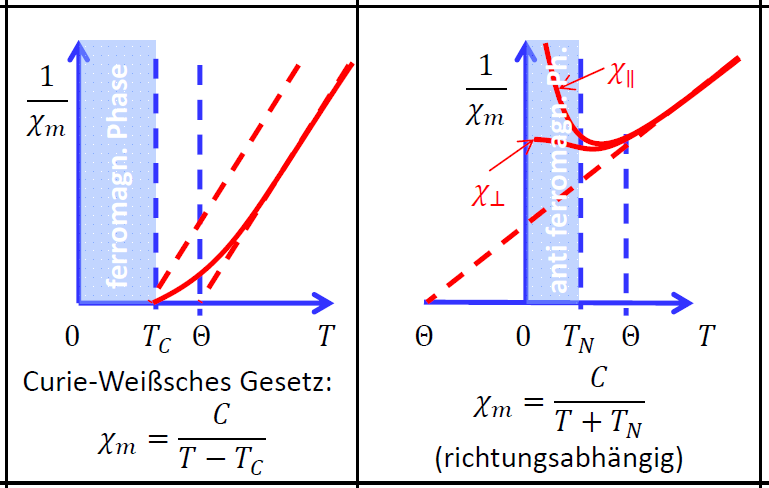
\includegraphics[width=18cm]{./aufgabe26.png}
  \caption{Dem Skript entnommen. Links: a) Ferromagnetismus. Rechts: b) Antiferromagnetismus}
\end{figure}


% \newpage

\end{document}

